\section{What Survives Synthetic-to-Real, and What Does Not}
\label{sec_disc_transfer}

The second cross-cutting finding is that the synthetic-to-real
distribution shift is one of the strongest determinants of performance
in this work.
Several configurations that perform well, or appear promising, on the
synthetic distribution lose part or all of that advantage when evaluated
on COCO.
Conversely, the largest improvement in the experimental chapter comes
not from introducing another architectural mechanism,
but from adapting the selected PG-GAT model to the COCO distribution
through fine-tuning.

This pattern appears across several experiments that otherwise have
little in common.
Removing the depth channel reduces synthetic performance but improves
zero-shot COCO transfer.
Fine-tuning PG-GAT on COCO produces a substantially larger improvement
than any individual PG-GAT modification.
The reduced-dimensional hyperbolic representation is competitive in the
synthetic-only setting but does not retain that advantage after COCO
fine-tuning.
TriGAT introduces articulation information that is meaningful in
principle,
yet performs worse after transfer,
while the visual-feature variant adds appearance information without
improving on the final position-and-type-only PG-GAT.
These experiments alter different parts of the pipeline,
but each exposes the same underlying difficulty -
a representation that is useful on the synthetic distribution is not
necessarily the representation that transfers best to real keypoint data.
Figure~\ref{fig:transfer_scatter} shows the pattern across every configuration in
Chapter~\ref{chap_4} that reports both numbers.

\begin{figure}[H]
    \centering
    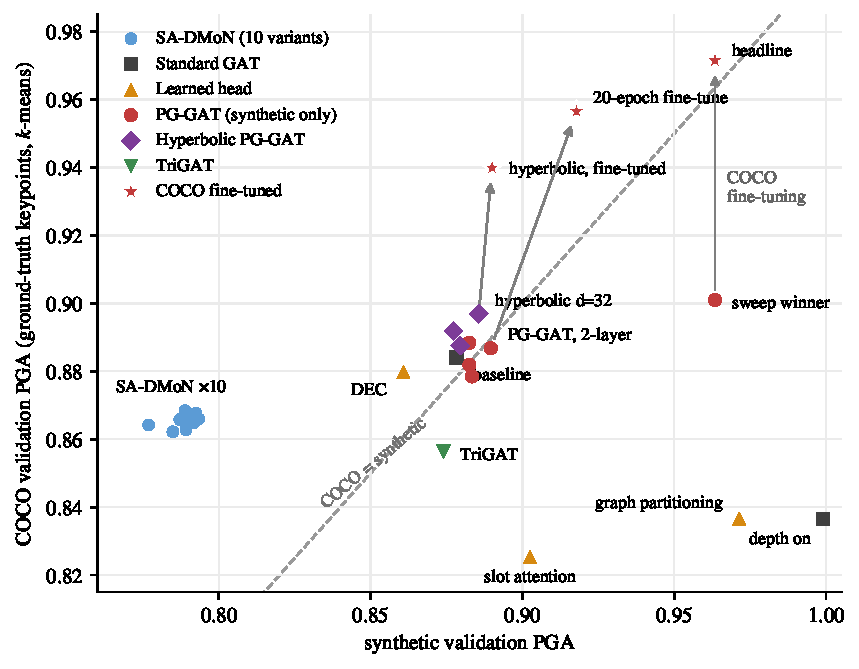
\includegraphics[width=0.92\linewidth]{figures/transfer_scatter.pdf}
    \caption[Synthetic-validation against COCO-validation PGA across the evaluated configurations.]{Synthetic-validation PGA against COCO-validation PGA
    using ground-truth keypoints and $k$-means
    for the 27 configurations in Chapter~\ref{chap_4} that report both metrics.
    The dashed diagonal represents equal performance on the two datasets;
    points below it perform worse on COCO than on the synthetic validation set,
    with the vertical distance from the diagonal indicating the transfer gap.
    Arrows connect the three synthetic-only models to their corresponding COCO fine-tuned versions,
    showing the change produced by real-data adaptation.
    Values are taken directly from the results reported in Chapter~\ref{chap_4}.
    TriGAT is evaluated on the $2{,}180$ scenes containing valid triplets,
    while all other configurations are evaluated on $2{,}307$ scenes.}
    \label{fig:transfer_scatter}
\end{figure}

The evidence therefore suggests that synthetic validation should be
treated primarily as a controlled environment for developing and
isolating architectural ideas,
rather than as a reliable predictor of their final COCO performance.
This distinction is important because the synthetic data remains useful
throughout the investigation.
It provides known person identities,
controlled scene composition,
and a repeatable setting in which individual design changes can be
compared without the additional variation introduced by a real detector.
The limitation is not that synthetic evaluation is uninformative,
but that improvements measured there cannot automatically be interpreted
as improvements in real-data grouping.

The remainder of this section examines this transfer effect through the
depth-removal experiment,
the COCO fine-tuning results,
and the hyperbolic,
TriGAT,
and visual-feature variants.
Considered together, these experiments show both sides of the same
problem -
features that make the synthetic task easier can become liabilities
after transfer,
while relatively modest adaptation to the target distribution can
produce larger gains than substantial changes to the model itself.
This distinction between \emph{synthetic discriminability} and
\emph{transferable discriminability} is central to interpreting the
experimental results that follow.

\subsection{Depth removal: the diagnostic that exposed the shift}
\label{sec_disc_transfer_depth}

The depth-removal diagnostic of Section~\ref{sec_res_baseline} provides
the clearest early evidence of the synthetic-to-real distribution shift.
With depth included, the standard GAT reaches a synthetic-validation
PGA of $0.9990$ but transfers to COCO at only $0.8366$.
Removing the depth channel reduces synthetic-validation PGA to $0.8783$,
a drop of $0.1207$,
while increasing COCO PGA to $0.8841$,
a gain of $0.0475$.
The direction of the two changes is more informative than either number
alone -
the feature that makes the synthetic grouping problem almost trivial is
also the feature that produces the weaker real-data representation.

The explanation lies in how depth is obtained in the two domains.
The synthetic generator of Section~\ref{sec_meth_data_synth} provides
metric depth from the Blender scene,
whereas the COCO pipeline of Section~\ref{sec_meth_data_coco} estimates
depth using MiDaS~\cite{ranftl2020midas}.
The latter provides relative depth rather than a metric camera-space
coordinate,
with scale and calibration that can vary between images.
A model trained on the synthetic depth channel can therefore exploit
relationships that are highly stable in the rendered data,
but are not represented in the same way at COCO inference time.
Removing depth sacrifices this particularly strong synthetic cue,
but also removes a source of distribution mismatch.

This result also explains why the depth-on synthetic configuration is a
poor setting in which to evaluate subsequent embedding modifications.
At $0.9990$ PGA there is almost no remaining grouping error for a new
architectural mechanism to correct.
The model can rely heavily on the metric depth coordinate to separate
people in three-dimensional scenes,
leaving little room for changes to the attention mechanism to produce a
measurable improvement.
Removing depth makes the synthetic problem harder,
but in doing so produces a more useful experimental setting for studying
whether the embedding network can learn person separation from signals
that are also available consistently on real data.

The depth-removal experiment therefore serves two purposes in the
methodology.
First, it motivates the no-depth configuration used by the subsequent
PG-GAT experiments.
Second, it establishes an important distinction for interpreting the
remainder of the results,
making the synthetic task easier is not equivalent to learning a
representation that transfers better.
A synthetic improvement is useful evidence only when the mechanism
responsible for that improvement remains meaningful under the
corresponding real-data distribution.
The experiments that follow repeatedly return to this distinction.

\subsection{COCO fine-tune: the largest lift in the pipeline}
\label{sec_disc_transfer_finetune}

The COCO fine-tuning experiment of Section~\ref{sec_res_coco_ft}
provides the clearest measurement of how strongly the target-data
distribution affects the final grouping result.
The synthetic-pretrained architecture-sweep winner reaches $0.9010$
COCO val PGA before fine-tuning and $0.9715$ after the fine-tune sweep,
an improvement of $0.0705$ on the same PG-GAT architecture.
This gain is substantially larger than the approximately $0.011$
improvement produced by combining the three PG-GAT modifications
at the matched baseline architecture
(Section~\ref{sec_disc_embedding_pggat}),
and is comparable in magnitude to the $0.0738$ improvement obtained
from the architecture sweep itself.
Adaptation to the target distribution is therefore one of the largest
individual effects measured in the experimental chapter.

Two aspects of this result help explain its significance.
First, the COCO improvement does not come at the expense of the
synthetic representation.
The fine-tuned checkpoint retains a synthetic-validation PGA of
$0.9634$,
equal to the value measured for the architecture-sweep checkpoint
before fine-tuning.
The corresponding synthetic-test result of $0.9580$ provides the same
general picture.
Within the resolution of these measurements,
the fine-tune therefore adapts the representation to COCO without
removing the person-separation structure learned during synthetic
pre-training.
The two stages appear complementary rather than competitive,
synthetic training establishes a useful grouping representation,
and COCO fine-tuning adjusts that representation to the statistics
of the target domain.

Second, relatively little additional performance is obtained by
optimising the fine-tuning recipe itself.
A 20-epoch fine-tune of the architecture-sweep winner reaches $0.9695$
COCO val PGA,
while the 12-run Bayesian sweep improves this to $0.9715$.
The difference of $0.0020$ is small relative to the variation of the
metric and should not be interpreted as a substantive gain.
Instead, the sweep shows that the inherited recipe lies within a
relatively flat region of the fine-tuning search space.
Its main contribution is therefore to support the choice of learning
rate,
weight decay,
and training duration rather than to provide another major source
of performance.

The contrast between these two effects is informative.
Changing the model's exposure from synthetic-only training to COCO
fine-tuning produces a $0.0705$ gain,
whereas searching over reasonable ways of performing that fine-tuning
produces only a further $0.0020$.
The important variable is therefore the target-domain data itself,
rather than a narrowly tuned optimisation schedule.
This reinforces the interpretation of the depth experiment -
representations learned from synthetic data can provide a strong
starting point,
but their final real-data performance depends heavily on whether the
information they encode remains appropriate for the target distribution.

This result provides the reference point for the architectural variants
considered next.
Hyperbolic embedding,
the triplet representation,
and visual-feature augmentation each introduce additional
representational structure that could, in principle, improve person
separation.
Their value cannot be judged from synthetic performance alone, however.
The more demanding question is whether the additional structure produces
an advantage once the model is evaluated or adapted on the real-data
distribution.
The results of those experiments show that this condition is
considerably harder to satisfy.

\subsection{Hyperbolic Option~B: the geometric prior loses to fine-tuning}
\label{sec_disc_transfer_hyperbolic}

The hyperbolic PG-GAT experiments of Section~\ref{sec_res_hyperbolic}
provide a useful example of an advantage that appears under
synthetic-only training but does not survive adaptation to the target
distribution.
Under H2, a $32$-dimensional hyperbolic embedding reaches $0.8856$
synthetic-validation PGA,
compared with $0.8896$ for the $128$-dimensional Euclidean ablation
model.
The difference is small relative to the variation of the metric,
so the result supports the intended efficiency interpretation -
in this setting, the hyperbolic representation retains approximately
the same grouping quality with a four-fold reduction in embedding
dimension.

The important test is whether that dimensional advantage persists once
the models are exposed to COCO.
Option~B fine-tunes the $32$-dimensional hyperbolic model and reaches
$0.9399$ COCO val PGA.
This is substantially higher than its synthetic-only COCO transfer
result of $0.8969$,
showing that the hyperbolic representation also benefits from
target-domain adaptation.
The improvement is not enough, however, to make it competitive with
the strongest Euclidean configurations.
It remains below the $0.9565$ legacy Euclidean fine-tune result and
$0.0316$ below the sweep-selected Euclidean headline of $0.9715$.
The dimensional efficiency observed in the synthetic-only experiment
therefore does not translate into a competitive fine-tuned COCO result.

One possible explanation is the scale of the hierarchy represented by
the pose graph.
The theoretical motivation for hyperbolic embeddings is strongest for
hierarchical and tree-like structures whose number of nodes grows
rapidly with depth,
where Euclidean representations require increasing dimension to
represent the structure with low distortion~\cite{sarkar2011treeembed}.
The COCO skeleton is small by comparison -
it contains only $17$ joint types and has a maximum topological depth
of only a few hops.
The pose-grouping problem may therefore provide too little hierarchical
structure for the geometric advantage of hyperbolic space to become
large at the embedding dimensions considered here.
This interpretation is consistent with the dim-$32$ result,
where hyperbolic geometry appears to preserve useful structure
efficiently,
but does not create a higher-quality representation than the larger
Euclidean model.

The fine-tuning results expose a second and empirically stronger effect.
The Euclidean PG-GAT gains $0.0705$ COCO PGA when the architecture-sweep
checkpoint is adapted from synthetic-only training to the final
COCO-fine-tuned configuration.
The hyperbolic Option~B model also improves after fine-tuning,
but its gain is smaller -
$0.8969$ to $0.9399$, or $0.0430$.
Whatever representational advantage the hyperbolic geometry provides
at low dimension is therefore not sufficient to compensate for the
stronger target-domain performance reached by the Euclidean model.
The experiment does not isolate whether this difference is caused by
embedding dimension,
manifold geometry,
optimisation behaviour,
or an interaction between them,
but it does establish that the synthetic efficiency result alone is not
predictive of the final COCO ranking.

The two pre-registered hypotheses should consequently be interpreted
separately.
H1, which predicts a quality advantage for hyperbolic embedding at
comparable dimension, is not supported by the experiments.
H2 receives partial support -
the $32$-dimensional hyperbolic model approximately matches the
$128$-dimensional Euclidean ablation model under synthetic-only training,
demonstrating that useful grouping structure can be represented at
substantially lower dimension.
That advantage does not survive strongly enough after COCO fine-tuning
to produce a competitive final model.
Hyperbolic PG-GAT is therefore best viewed as an efficiency observation
under the synthetic regime,
rather than as an alternative to the Euclidean headline configuration.

\subsection{TriGAT: a richer primitive whose downstream voting step is lossy}
\label{sec_disc_transfer_trigat}

TriGAT (Section~\ref{sec_res_trigat}) explores a different alternative
to the standard PG-GAT formulation.
Rather than changing the embedding geometry or adding another feature
source, it changes the graph primitive from individual joints to
triplets of three connected joints.
The motivation is that a triplet provides local articulation information
through its pivot angle,
which is invariant to global rotation and is not directly available
from the position of a single joint.
Under the matched synthetic training regime, however,
TriGAT reaches $0.8740$ synthetic-validation PGA compared with $0.8896$
for the corresponding PG-GAT ablation configuration,
a difference of $-0.0156$.

The main weakness of the implemented formulation appears in the
conversion from triplet-level clusters back to joint-level assignments.
A joint can belong to several overlapping triplets,
and those triplets are not guaranteed to receive the same cluster label
after $k$-means.
The weighted-majority rule of Section~\ref{sec_meth_trigat_voting}
must therefore reconcile potentially inconsistent triplet assignments
before the final joint partition can be formed.
This introduces an additional inference step that is absent from the
joint-based PG-GAT pipeline.

Errors at the triplet level can also propagate through this conversion.
A mis-clustered triplet contains three joints and overlaps with
neighbouring triplets,
so its incorrect assignment can influence the final labels of several
joints.
The voting rule can correct an isolated error when the remaining
triplets agree,
but it cannot recover reliably when several overlapping assignments
disagree.
The additional articulation information must therefore provide enough
improvement in the triplet embedding to compensate for the error
introduced by the subsequent voting stage.
The measured result indicates that this does not happen in the present
architecture.

This result does not show that articulation is an unhelpful cue.
The triplet representation explicitly contains pivot-angle information
that is absent from the single-joint input,
and the pivot angle is a rotation-invariant descriptor of local
articulation.
Instead, the experiment shows that the implemented route for exploiting
this information loses more during the triplet-to-joint conversion than
it gains from the richer representation.
The negative result therefore applies to the combination of triplet-level
embedding,
triplet-level clustering,
and joint-level voting rather than to the articulation signal itself.

A natural follow-on would be to retain the articulation information
while avoiding the intermediate triplet clustering.
For example, overlapping triplet embeddings could be aggregated into a
joint-level representation before clustering,
or a learned mapping could predict joint assignments directly from the
surrounding triplet representations.
Either approach would preserve the joint as the final grouping primitive
while still allowing local articulation to contribute to its embedding.
These alternatives require a different architecture and are therefore
left for future work.

The TriGAT experiment consequently answers the graph-primitive question
more narrowly than a simple comparison between joints and triplets might
suggest.
Changing to a richer primitive does not improve grouping merely because
that primitive contains additional information -
the architecture must also preserve that information through to the
final joint-level decision.
For the TriGAT formulation evaluated here,
the evidence points to the triplet-to-joint voting stage as the main
bottleneck,
making the implemented design a documented negative result rather than
evidence against articulation-based features more generally.


\subsection{PG-GAT v2: visual features do not beat the sweep-defended baseline}
\label{sec_disc_transfer_v2}

The PG-GAT v2 experiment tests whether appearance information can add
useful identity cues beyond the position-and-type representation used by
the standard PG-GAT (Section~\ref{sec_res_v2}).
Pre-trained MobileNetV2 features are sampled at each keypoint location
and projected into the node representation before message passing.
The 20-epoch configuration reaches $0.9670$ COCO val PGA,
while extending training to 50 epochs raises this to $0.9682$.
Both remain below the \texttt{meng-headline} result of $0.9715$,
by $0.0045$ and $0.0033$ respectively.
The additional visual information therefore does not produce a better
operating point in the configuration evaluated here.

This result is consistent with the diminishing returns observed in the
earlier feasibility experiments.
When MobileNetV2 features were added to a simple position-based
$k$-means representation, the improvement was approximately $+0.07$
COCO PGA.
As the underlying representation became stronger, however,
the additional gain from the same visual signal became much smaller.
This suggests that appearance features are most useful when the existing
representation contains relatively little identity information.
Once position, joint type, skeleton structure, and learned message
passing already provide a strong separation between people, much of the
useful information supplied by the visual features may be redundant.

The fully trained v2 experiment follows this pattern.
PG-GAT already uses joint type and relative skeleton structure to
organise the embedding,
and COCO fine-tuning adapts that representation directly to the target
distribution.
At this operating point, adding generic ImageNet features does not
improve the final PGA.
This does not imply that the visual features contain no identity
information - the earlier feasibility result shows that they do.
Rather, their marginal contribution decreases as the non-visual
embedding becomes stronger.
The additional signal is not sufficient to produce an improvement over
the sweep-selected and COCO-fine-tuned PG-GAT configuration.

There is an important qualification to this comparison.
PG-GAT v2 extends the legacy two-layer architecture rather than the
architecture-sweep-selected three-layer headline model.
The experiment therefore does not isolate the marginal effect of adding
visual features to the exact \texttt{meng-headline} architecture.
A fully matched ablation would require adding the same visual pathway
to the sweep-selected PG-GAT and repeating the fine-tune procedure.
The present result supports the narrower conclusion that the implemented
v2 configuration does not provide a better practical operating point
than the final position-and-type model -
it does not establish that visual features could never improve a
stronger or differently trained PG-GAT.

The computational cost makes the measured trade less attractive.
The v2 network contains approximately $27{,}000$ additional parameters
relative to the legacy two-layer PG-GAT that it extends,
and the frozen MobileNetV2 feature extractor contributes a further
approximately $2.2 \times 10^{6}$ parameters.
More importantly, the MobileNetV2 backbone must be executed at
inference time because its feature maps are required to construct the
visual node features.
When combined with the HigherHRNet detector and PG-GAT v2 network,
the resulting deployable pipeline contains approximately
$31.0 \times 10^{6}$ parameters,
compared with approximately $28.6 \times 10^{6}$ for HigherHRNet alone.

The added computation is not accompanied by an accuracy gain in the
experiments reported here.
The extended v2 configuration reaches $0.9682$ COCO val PGA,
below the $0.9715$ no-visual-feature PG-GAT headline.
The HigherHRNet AE figure of $0.9847$ is also higher,
although that value is an end-to-end PGA measured on matched detector
outputs and should not be treated as a strictly like-for-like comparison
with the ground-truth-keypoint v2 value.
It is nevertheless relevant to the deployment trade -
the visual pathway increases the total system size without closing the
accuracy gap to the native detector-specific grouping mechanism.

The experiment therefore provides a negative result for the visual
augmentation implemented in PG-GAT v2.
Appearance features are useful when added to a weak positional
representation,
but their marginal value decreases as the underlying embedding improves.
At the operating points tested here,
the additional MobileNetV2 pathway increases model size and inference
requirements without exceeding the simpler PG-GAT headline.
For that reason, visual augmentation is not pursued further in this
work.
A future investigation could revisit the idea using a matched
sweep-selected architecture,
detector-native visual features,
or jointly trained appearance features,
but those experiments would test a different formulation from the frozen
ImageNet feature pathway evaluated here.

\subsection{Synthesis}
\label{sec_disc_transfer_synthesis}

Reading Sections~\ref{sec_disc_transfer_depth}--\ref{sec_disc_transfer_v2}
together shows that the synthetic-to-real shift affects each of the
alternative representations in a different way.
The depth-on baseline is the clearest example -
near-perfect synthetic performance falls to $0.8366$ on COCO because
the depth signal changes between the two domains.
The low-dimensional hyperbolic model retains useful structure
efficiently under synthetic training,
but its advantage is not sufficient to remain competitive after COCO
fine-tuning.
TriGAT introduces articulation information but loses more through its
triplet-to-joint voting stage than it gains from the richer primitive.
The visual-feature variant adds appearance information at considerable
computational cost,
yet the implemented configuration remains below the
position-and-type-only headline model.
Although the mechanisms differ, the common result is that an advantage
observed or motivated in the controlled setting does not automatically
translate into an advantage at the final COCO operating point.

The COCO fine-tuning experiment provides the strongest counterpoint.
Adapting the architecture-sweep-selected PG-GAT from synthetic training
to COCO increases COCO val PGA from $0.9010$ to $0.9715$,
a gain of $0.0705$,
while preserving its $0.9634$ synthetic-validation PGA.
This improvement is comparable to the gain produced by the architecture
sweep itself and larger than the changes associated with the individual
architectural alternatives considered in this section.
The result therefore identifies exposure to the target distribution
as a major determinant of real-data grouping performance,
rather than treating synthetic performance as a sufficient proxy for it.

This provides the experimental answer to \emph{RQ6: synthetic-to-real
transfer}.
Synthetic data provides a useful environment for isolating architectural
effects and learning an initial person-separation representation,
but performance measured there is not by itself a reliable predictor
of the final COCO ranking.
Features that are highly discriminative in the synthetic domain can
transfer poorly when their statistics change,
as demonstrated most directly by depth.
Conversely, a representation that is already strong on synthetic data
can still gain substantially when adapted to the target distribution.
The synthetic and real stages should therefore be treated as complementary,
the former supports controlled architectural development,
while the latter is necessary to establish whether the resulting
representation remains useful under realistic data.

This finding also constrains the answers to \emph{RQ4: embedding
geometry} and \emph{RQ5: graph primitive}.
For RQ4, the hyperbolic experiments provide evidence that a
lower-dimensional representation can retain comparable grouping
information under synthetic-only training,
but they do not establish a quality advantage over the Euclidean
embedding at the final COCO operating point.
The result is therefore best interpreted as an efficiency observation,
rather than as evidence for replacing the Euclidean headline model.
For RQ5, the TriGAT result shows that introducing articulation through
a triplet primitive does not improve grouping in the architecture
evaluated here.
The negative result is associated with the additional triplet-clustering
and voting stage,
rather than demonstrating that articulation itself is uninformative.

The visual-feature experiment provides a related negative result.
The implemented MobileNetV2 augmentation reaches $0.9682$ COCO val PGA,
compared with $0.9715$ for the no-visual-feature headline model,
while requiring an additional visual feature extractor at inference.
Because the v2 experiment uses the legacy two-layer architecture rather
than the sweep-selected headline architecture,
it does not isolate the marginal effect of appearance features on the
final PG-GAT configuration.
It does, however, show that the implemented visual pathway does not
provide a better practical operating point than the simpler
position-and-type model.

The methodological consequence is not that architectural alternatives
are unimportant,
but that they must be judged after the relevant domain shift rather
than by their synthetic behaviour alone.
In the experiments reported here, the most reliable path to the final
result is to retain the skeleton-aware PG-GAT representation selected
by the architecture sweep and then adapt that representation to COCO.
The architecture sweep determines a model with sufficient capacity
to exploit the pose-specific inductive biases,
while the fine-tuning stage adapts those features to the target
distribution.
The headline result is the product of these two stages,
architecture selection establishes the representation,
and target-domain fine-tuning makes that representation effective
on real data.